\documentclass[12pt,a4paper]{report}

% ==================== 宏包 ====================
\usepackage[UTF8]{ctex}
\usepackage{geometry}
\geometry{left=2.5cm, right=2.5cm, top=3cm, bottom=3cm}

\usepackage{graphicx}
\usepackage{booktabs}
\usepackage{longtable}
\usepackage{array}
\usepackage{enumitem}
\usepackage{listings}
\usepackage{xcolor}
\usepackage{tikz}
\usetikzlibrary{shapes, arrows.meta, positioning, fit, backgrounds, calc}
\usepackage{hyperref}
\usepackage{tocloft}
\usepackage{fancyhdr}
\usepackage{titlesec}
\usepackage{multirow}
\usepackage{tabularx}
\usepackage{makecell}
\usepackage{amsmath}
\usepackage{amssymb}

% ==================== 样式 ====================
\hypersetup{
    colorlinks=true,
    linkcolor=black!70,
    citecolor=blue!60!black,
    urlcolor=blue!60!black
}

\titleformat{\chapter}[hang]{\centering\Huge\bfseries}{第\chinese{chapter}章}{1em}{}
\titleformat{\section}{\Large\bfseries}{\thesection}{1em}{}
\titleformat{\subsection}{\large\bfseries}{\thesubsection}{1em}{}

\pagestyle{fancy}
\fancyhf{}
\fancyhead[C]{\small 基于智能体的个性化旅游系统 --- 系统架构设计文档}
\fancyfoot[C]{\thepage}
\renewcommand{\headrulewidth}{0.4pt}
\renewcommand{\footrulewidth}{0.4pt}

\lstset{
    basicstyle=\ttfamily\small,
    keywordstyle=\color{blue}\bfseries,
    commentstyle=\color{green!50!black},
    stringstyle=\color{red!60!black},
    numbers=left,
    numberstyle=\tiny\color{gray},
    frame=single,
    breaklines=true,
    tabsize=4
}

% ==================== 封面 ====================
\begin{document}

\begin{titlepage}
\centering
\vspace*{3cm}

{\Huge\bfseries 基于智能体的个性化旅游系统}

\vspace{1.5cm}

{\LARGE\bfseries 系统架构设计文档}

\vspace{2cm}

\rule{\textwidth}{1pt}

\vspace{1cm}

{\Large 数据结构课程设计}

\vspace{0.5cm}

{\large 北京邮电大学计算机学院}

\vspace{0.3cm}

{\large 2026年3月}

\vspace{1cm}

\rule{\textwidth}{1pt}

\vspace{2cm}

{\large
\begin{tabular}{rl}
课程名称： & 数据结构课程设计 \\
适用班级： & 309\textasciitilde312 \\
指导教师： & 郭岗 \\
\end{tabular}
}

\end{titlepage}

% ==================== 目录 ====================
\tableofcontents
\newpage

% ====================================================================
% 第1章  项目概述
% ====================================================================
\chapter{项目概述}

\section{项目背景}

本项目为北京邮电大学计算机学院数据结构课程设计项目。随着旅游业的快速发展，大学生群体对个性化旅游服务的需求日益增长。现有的旅游平台往往功能单一，无法提供从旅游前目的地推荐、旅游中路线规划到旅游后日记交流的一站式服务。

本系统利用智能体（Agent）辅助完成系统设计与开发，核心考查数据结构与算法的设计与实现能力。项目周期为2026年3月至2026年6月，采用3人小组协作模式。

\section{项目目标}

本系统旨在构建一个面向大学生旅游场景的个性化旅游系统，提供以下全流程服务：

\begin{enumerate}[label=(\arabic*)]
    \item \textbf{旅游前}：按照旅游目的地的热度、评价和个人兴趣选择和推荐旅游目的地
    \item \textbf{旅游中}：在景区或校园内规划最优参观路线，提供景点介绍和场所查询
    \item \textbf{旅游后}：根据游览经历生成旅游日记，支持社区交流与分享
\end{enumerate}

\section{设计原则}

\begin{itemize}
    \item \textbf{算法核心}：所有核心算法必须基于自己设计的数据结构，自己编程实现，这是课程考查重点
    \item \textbf{模块化设计}：清晰的模块边界和接口定义，便于3人分工协作
    \item \textbf{前后端分离}：C++负责算法引擎与后端服务，Vue 3负责图形化展示
    \item \textbf{可扩展性}：预留接口，支持后续功能迭代
    \item \textbf{简洁实用}：面向初学者团队，避免过度设计
\end{itemize}


% ====================================================================
% 第2章  需求分析
% ====================================================================
\chapter{需求分析}

\section{功能需求概述}

系统包含6大核心功能模块：

\begin{enumerate}
    \item \textbf{旅游推荐}：按热度/评价/个人兴趣推荐景点和学校，支持Top-K不完全排序和关键字模糊查询
    \item \textbf{旅游路线规划}：单目标最短路径（Dijkstra）、多目标TSP路径、拥挤度策略、交通工具混合、室内导航
    \item \textbf{场所查询}：基于实际可达路径距离的周边设施查找与排序（非直线距离）
    \item \textbf{旅游日记管理}：文字/图片/视频日记撰写、浏览量热度、评分排序
    \item \textbf{旅游日记交流}：目的地关联查找、精确查询（哈希）、全文检索（Trie/倒排索引）、Huffman无损压缩存储、AIGC动画生成
    \item \textbf{美食推荐}：Top-K排序、菜系过滤、模糊查询（编辑距离）
\end{enumerate}

\section{核心算法需求}

下表汇总了各功能模块对应的核心算法、自定义数据结构及复杂度要求：

\begin{table}[H]
\centering
\caption{核心算法需求总表}
\small
\begin{tabularx}{\textwidth}{>{\centering}p{2.8cm} >{\centering}p{3.5cm} >{\centering}p{3.5cm} X}
\toprule
\textbf{功能模块} & \textbf{核心算法} & \textbf{自定义数据结构} & \textbf{复杂度要求} \\
\midrule
旅游推荐 & Top-K堆排序 & MaxHeap（堆） & $O(n + k \log n)$，不完全排序 \\
美食推荐 & Top-K堆排序 & MaxHeap（堆） & $O(n + k \log n)$，不完全排序 \\
路线规划（单目标） & Dijkstra & 邻接表AdjList，优先队列 & $O((V+E) \log V)$ \\
路线规划（多目标） & TSP近似（最近邻+2-opt） & 图，路径集合 & $O(n^2)$ 近似解 \\
拥挤度最短时间 & Dijkstra变体 & 加权边（时间权重） & $O((V+E) \log V)$ \\
交通工具混合 & 多层图Dijkstra & 多层邻接表 & $O((V+E) \log V)$ \\
场所查询 & Dijkstra + BFS & 图，设施分类链表 & 依赖Dijkstra求路径距离 \\
日记精确查询 & 哈希表查找 & HashMap & $O(1)$ 平均查找 \\
日记全文检索 & Trie / 倒排索引 & Trie树，InvertedIndex & $O(m)$，$m$为关键词长度 \\
日记压缩存储 & Huffman编码 & Huffman树，编码表 & $O(n \log n)$ 构建 \\
美食模糊查询 & 编辑距离 & 动态规划表 & $O(m \times n)$ \\
\bottomrule
\end{tabularx}
\end{table}

\section{数据规模要求}

\begin{table}[H]
\centering
\caption{数据规模要求}
\begin{tabular}{lc}
\toprule
\textbf{数据项} & \textbf{最低要求} \\
\midrule
景区/校园数量 & $\geq 200$ 个 \\
每处建筑物数量 & $\geq 20$ 个 \\
服务设施种类 & $\geq 10$ 种 \\
服务设施数量 & $\geq 50$ 个 \\
道路边数 & $\geq 200$ 条 \\
系统用户数 & $\geq 10$ 人 \\
\bottomrule
\end{tabular}
\end{table}


% ====================================================================
% 第3章  技术选型
% ====================================================================
\chapter{技术选型}

\section{技术栈总览}

\begin{table}[H]
\centering
\caption{技术栈选型总表}
\begin{tabularx}{\textwidth}{>{\centering}p{2.2cm} X >{\centering}p{4.5cm}}
\toprule
\textbf{层级} & \textbf{技术} & \textbf{选型理由} \\
\midrule
核心语言 & C++17 & 课程核心考查算法，C++实现算法最直观、性能最优 \\
HTTP服务 & cpp-httplib & 零依赖单头文件库，初学者友好，支持REST API \\
JSON处理 & nlohmann/json & 零依赖单头文件库，C++最流行的JSON库 \\
数据库 & SQLite3 & 零配置单文件数据库，C++通过C API直接操作 \\
构建系统 & CMake & C++工业标准，跨平台，依赖管理清晰 \\
前端框架 & Vue 3 + Vite & 组合式API简洁，Vite开发体验好，生态丰富 \\
UI组件库 & Element Plus & Vue 3生态最成熟的中文友好组件库 \\
地图可视化 & HTML5 Canvas & 简化版节点+连线展示，无需外部地图API \\
HTTP客户端 & Axios & 前端调用后端REST API，拦截器封装方便 \\
\bottomrule
\end{tabularx}
\end{table}

\section{选型对比分析}

\subsection{核心语言：为何选择C++}

\begin{itemize}
    \item \textbf{课程匹配}：数据结构课程以C++为主要教学语言，算法实现更贴合课程要求
    \item \textbf{性能优势}：图算法、排序算法等计算密集型任务，C++执行效率远高于解释型语言
    \item \textbf{内存控制}：自定义数据结构（邻接表、堆、Trie、哈希表）需要精细的内存管理
    \item \textbf{评分优势}：答辩时可以直接展示算法实现的底层细节，体现对数据结构的理解
\end{itemize}

\textbf{未选方案}：Python（算法实现不够底层，不符合课程考查意图）、Java（模板代码过多，初学者上手慢）。

\subsection{HTTP服务：为何选择cpp-httplib}

\begin{itemize}
    \item \textbf{零配置}：单头文件引入，无需编译安装依赖库
    \item \textbf{API简洁}：类似Python Flask的链式调用风格，学习成本低
    \item \textbf{静态文件托管}：内置静态文件服务，可直接托管Vue前端构建产物
\end{itemize}

\textbf{未选方案}：Crow（依赖Boost，编译复杂）、Pistache（C++11，API较繁琐）。

\subsection{数据库：为何选择SQLite}

\begin{itemize}
    \item \textbf{零安装}：无需数据库服务器进程，单文件存储
    \item \textbf{C API直接调用}：C++可直接链接sqlite3库，无ORM中间层
    \item \textbf{适合课程设计}：数据规模适中，SQLite完全胜任
\end{itemize}

\textbf{未选方案}：MySQL/PostgreSQL（需安装配置，过重）、MongoDB（文档型，关系数据不友好）。


% ====================================================================
% 第4章  系统架构设计
% ====================================================================
\chapter{系统架构设计}

\section{架构模式}

本系统采用\textbf{模块化单体分层架构}。对于3人初学者团队，模块化单体是最务实的选择：它提供了清晰的模块边界便于分工，同时避免了微服务带来的分布式复杂性。系统整体分为五层，职责清晰，依赖方向单一。

\section{系统架构图}

\begin{figure}[H]
\centering
\begin{tikzpicture}[
    node distance=0.8cm,
    layer/.style={
        draw, rounded corners, minimum width=14cm, minimum height=1.4cm,
        font=\small\bfseries, align=center, fill=#1
    },
    module/.style={
        draw, rounded corners, minimum width=2.4cm, minimum height=0.7cm,
        font=\footnotesize, align=center, fill=#1
    },
    arr/.style={-{Stealth[length=3mm]}, thick, color=black!60}
]

% Layers
\node[layer=blue!10] (frontend) at (0, 5) {表示层（Vue 3 前端）};
\node[layer=green!10] (api) at (0, 3.2) {接口层（REST API 路由层 --- cpp-httplib）};
\node[layer=orange!10] (service) at (0, 1.4) {业务逻辑层（Service）};
\node[layer=red!10] (algo) at (0, -0.4) {算法引擎层（Algorithm --- 课程核心）};
\node[layer=purple!10] (data) at (0, -2.2) {数据访问层（Repository / DAO）};

% Database
\node[draw, cylinder, shape border rotate=90, aspect=0.25,
      minimum width=3cm, minimum height=1.2cm, fill=gray!15,
      font=\small\bfseries] (db) at (0, -4) {SQLite 数据库};

% Arrows
\draw[arr] (frontend) -- (api);
\draw[arr] (api) -- (service);
\draw[arr] (service) -- (algo);
\draw[arr] (service) -- (data);
\draw[arr] (algo) -- (data);
\draw[arr] (data) -- (db);

% Frontend modules
\node[module=blue!20] at (-5, 5) {推荐页面};
\node[module=blue!20] at (-2.5, 5) {地图导航};
\node[module=blue!20] at (0, 5) {场所查询};
\node[module=blue!20] at (2.5, 5) {日记管理};
\node[module=blue!20] at (5, 5) {美食推荐};

% Service modules
\node[module=orange!20] at (-4.5, 1.4) {推荐服务};
\node[module=orange!20] at (-1.5, 1.4) {路线服务};
\node[module=orange!20] at (1.5, 1.4) {场所服务};
\node[module=orange!20] at (4.5, 1.4) {日记服务};

% Algorithm modules
\node[module=red!15] at (-5.5, -0.4) {MaxHeap};
\node[module=red!15] at (-3.3, -0.4) {Dijkstra};
\node[module=red!15] at (-1.1, -0.4) {TSP};
\node[module=red!15] at (1.1, -0.4) {HashMap};
\node[module=red!15] at (3.3, -0.4) {Trie};
\node[module=red!15] at (5.5, -0.4) {Huffman};

\end{tikzpicture}
\caption{系统分层架构图}
\end{figure}

\section{各层职责说明}

\subsection{表示层（Vue 3 前端）}

\begin{itemize}
    \item 负责页面渲染、用户交互、数据展示
    \item Canvas绘制简化版路网地图和路径可视化
    \item 通过Axios发送HTTP请求调用后端API
    \item 5个核心页面：推荐页、地图导航页、场所查询页、日记页、美食推荐页
\end{itemize}

\subsection{接口层（REST API 路由层）}

\begin{itemize}
    \item 基于cpp-httplib实现HTTP路由注册
    \item 负责请求参数解析、校验
    \item JSON请求体解析和JSON响应序列化
    \item 统一错误处理和响应格式
\end{itemize}

\subsection{业务逻辑层（Service）}

\begin{itemize}
    \item 编排业务流程，协调算法引擎和数据访问
    \item 不包含具体算法实现，只负责调用和组装
    \item 5个服务模块对应5大功能：RecommendService、RouteService、FacilityService、DiaryService、FoodService
\end{itemize}

\subsection{算法引擎层（Algorithm --- 课程核心）}

\begin{itemize}
    \item 纯算法逻辑，\textbf{无IO依赖}，便于独立测试
    \item 所有数据结构均为自定义实现，不使用STL容器（课程要求）
    \item 9个算法模块：Graph、Heap、Dijkstra、TSP、HashMap、Trie、InvertedIndex、Huffman、EditDistance
\end{itemize}

\subsection{数据访问层（Repository / DAO）}

\begin{itemize}
    \item 封装所有SQLite数据库操作（CRUD）
    \item 提供统一的数据访问接口
    \item 5个Repository：SpotRepo、RouteRepo、FacilityRepo、DiaryRepo、FoodRepo
\end{itemize}

\section{数据流向}

\begin{center}
\begin{tikzpicture}[node distance=0.3cm, font=\footnotesize,
    box/.style={draw, rounded corners, fill=gray!10, minimum height=0.6cm, minimum width=1.8cm, align=center}]
\node[box] (user) {用户操作};
\node[box, right=of user] (vue) {Vue组件};
\node[box, right=of vue] (axios) {Axios请求};
\node[box, right=of axios] (httplib) {cpp-httplib};
\node[box, below=0.5cm of httplib] (service) {Service层};
\node[box, left=of service] (algo) {Algorithm层};
\node[box, right=of service] (repo) {Repository层};
\node[box, below=0.5cm of repo] (sqlite) {SQLite};
\node[box, left=of sqlite] (json) {JSON序列化};
\node[box, left=of json] (resp) {HTTP响应};
\node[box, left=of resp] (render) {Vue渲染};

\draw[-{Stealth}, thick] (user) -- (vue);
\draw[-{Stealth}, thick] (vue) -- (axios);
\draw[-{Stealth}, thick] (axios) -- (httplib);
\draw[-{Stealth}, thick] (httplib) -- (service);
\draw[-{Stealth}, thick] (service) -- (algo);
\draw[-{Stealth}, thick] (service) -- (repo);
\draw[-{Stealth}, thick] (repo) -- (sqlite);
\draw[-{Stealth}, thick, dashed] (sqlite) -- (json) -- (resp) -- (render) -- (vue);
\end{tikzpicture}
\end{center}

\section{前后端集成方式}

\begin{itemize}
    \item \textbf{开发阶段}：前端Vite dev server配置代理，将API请求转发到C++后端端口（默认8080）
    \item \textbf{生产阶段}：C++后端通过cpp-httplib的\texttt{set\_mount\_point("/", "./dist")}直接托管Vue前端构建产物，只需启动一个进程即可访问完整系统
    \item \textbf{跨域处理}：开发时通过Vite proxy解决，生产时同源无跨域问题
\end{itemize}


% ====================================================================
% 第5章  模块设计
% ====================================================================
\chapter{模块设计}

\section{后端模块划分}

\begin{table}[H]
\centering
\caption{后端项目目录结构}
\small
\begin{tabularx}{\textwidth}{X l}
\toprule
\textbf{目录/文件} & \textbf{说明} \\
\midrule
\texttt{CMakeLists.txt} & CMake构建配置 \\
\texttt{third\_party/httplib.h} & cpp-httplib头文件（header-only） \\
\texttt{third\_party/json.hpp} & nlohmann/json头文件（header-only） \\
\midrule
\texttt{include/server/http\_server.h} & HTTP服务器启动与路由注册 \\
\texttt{include/server/response.h} & 统一响应格式封装 \\
\texttt{include/service/recommend\_service.h} & 旅游推荐业务逻辑 \\
\texttt{include/service/route\_service.h} & 路线规划业务逻辑 \\
\texttt{include/service/facility\_service.h} & 场所查询业务逻辑 \\
\texttt{include/service/diary\_service.h} & 日记管理业务逻辑 \\
\texttt{include/service/food\_service.h} & 美食推荐业务逻辑 \\
\texttt{include/algorithm/graph.h} & 邻接表图数据结构 \\
\texttt{include/algorithm/heap.h} & 最大堆/最小堆（Top-K） \\
\texttt{include/algorithm/dijkstra.h} & Dijkstra最短路径 \\
\texttt{include/algorithm/tsp.h} & TSP近似算法 \\
\texttt{include/algorithm/hash\_table.h} & 哈希表（精确查找） \\
\texttt{include/algorithm/trie.h} & Trie树（全文检索） \\
\texttt{include/algorithm/inverted\_index.h} & 倒排索引 \\
\texttt{include/algorithm/huffman.h} & Huffman编码压缩 \\
\texttt{include/algorithm/edit\_distance.h} & 编辑距离（模糊查询） \\
\texttt{include/repository/db\_connection.h} & SQLite连接管理 \\
\texttt{include/repository/spot\_repo.h} & 景点数据访问 \\
\texttt{include/repository/route\_repo.h} & 路网数据访问 \\
\texttt{include/repository/facility\_repo.h} & 设施数据访问 \\
\texttt{include/repository/diary\_repo.h} & 日记数据访问 \\
\texttt{include/repository/food\_repo.h} & 美食数据访问 \\
\texttt{include/models/} & 数据模型定义（spot.h, building.h等） \\
\midrule
\texttt{src/main.cpp} & 程序入口 \\
\texttt{src/server/route\_handlers.cpp} & API路由处理函数 \\
\texttt{src/data/data\_loader.cpp} & 初始化数据加载 \\
\texttt{data/init\_db.sql} & 数据库初始化SQL \\
\texttt{tests/} & 算法单元测试 \\
\bottomrule
\end{tabularx}
\end{table}

\section{前端模块划分}

\begin{table}[H]
\centering
\caption{前端项目目录结构}
\small
\begin{tabularx}{\textwidth}{X l}
\toprule
\textbf{目录/文件} & \textbf{说明} \\
\midrule
\texttt{src/views/HomeView.vue} & 首页---旅游推荐 \\
\texttt{src/views/MapView.vue} & 地图导航---路线规划 \\
\texttt{src/views/FacilityView.vue} & 场所查询 \\
\texttt{src/views/DiaryView.vue} & 旅游日记管理与交流 \\
\texttt{src/views/FoodView.vue} & 美食推荐 \\
\texttt{src/components/} & 通用组件（NavBar, SpotCard, MapCanvas等） \\
\texttt{src/api/} & API调用模块（spot.js, route.js等） \\
\texttt{src/router/index.js} & Vue Router路由配置 \\
\texttt{src/utils/request.js} & Axios封装（拦截器、统一错误处理） \\
\texttt{src/stores/} & Pinia状态管理 \\
\bottomrule
\end{tabularx}
\end{table}

\section{模块依赖关系}

\begin{figure}[H]
\centering
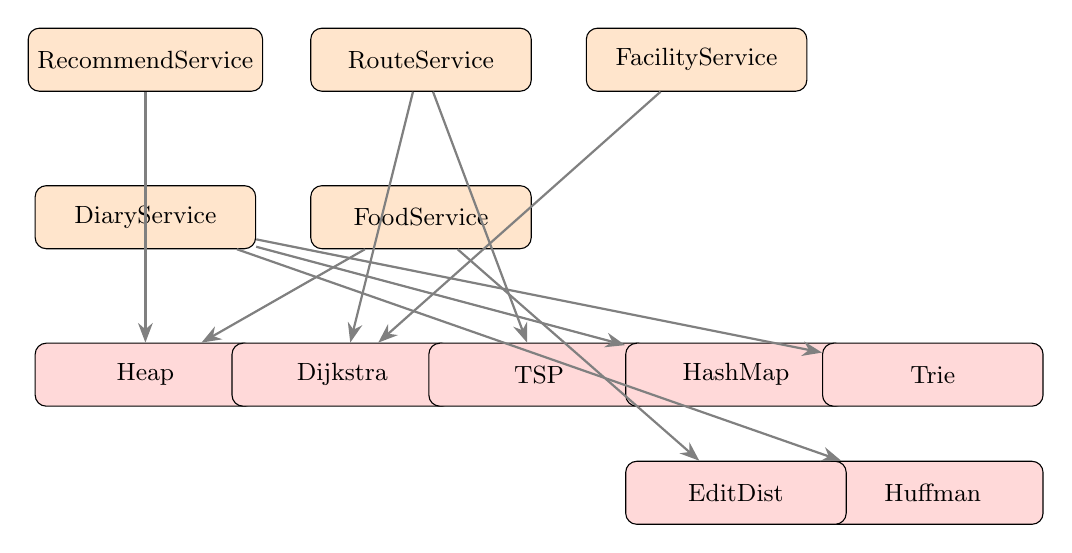
\begin{tikzpicture}[
    node distance=1cm,
    mod/.style={draw, rounded corners, minimum width=2.8cm, minimum height=0.8cm,
                font=\small, align=center, fill=#1},
    dep/.style={-{Stealth[length=2.5mm]}, thick, color=black!50}
]
% Service layer
\node[mod=orange!20] (rec) at (0, 3) {RecommendService};
\node[mod=orange!20] (rou) at (3.5, 3) {RouteService};
\node[mod=orange!20] (fac) at (7, 3) {FacilityService};
\node[mod=orange!20] (dia) at (0, 1) {DiaryService};
\node[mod=orange!20] (foo) at (3.5, 1) {FoodService};

% Algorithm layer
\node[mod=red!15] (heap) at (0, -1) {Heap};
\node[mod=red!15] (dijk) at (2.5, -1) {Dijkstra};
\node[mod=red!15] (tsp) at (5, -1) {TSP};
\node[mod=red!15] (hash) at (7.5, -1) {HashMap};
\node[mod=red!15] (trie) at (10, -1) {Trie};
\node[mod=red!15] (huff) at (10, -2.5) {Huffman};
\node[mod=red!15] (edit) at (7.5, -2.5) {EditDist};

% Dependencies
\draw[dep] (rec) -- (heap);
\draw[dep] (rou) -- (dijk);
\draw[dep] (rou) -- (tsp);
\draw[dep] (fac) -- (dijk);
\draw[dep] (dia) -- (hash);
\draw[dep] (dia) -- (trie);
\draw[dep] (dia) -- (huff);
\draw[dep] (foo) -- (heap);
\draw[dep] (foo) -- (edit);
\end{tikzpicture}
\caption{Service层与Algorithm层依赖关系}
\end{figure}


% ====================================================================
% 第6章  数据结构设计
% ====================================================================
\chapter{数据结构设计}

本章详细描述系统所需的自定义数据结构。所有数据结构均为\textbf{自行实现}，不使用STL容器（除iostream等基础库外），以满足课程设计要求。

\section{邻接表图（AdjacencyList）}

\subsection{用途}
表示景区/校园内部道路路网，支持Dijkstra最短路径、TSP路径规划、场所距离查询等算法。

\subsection{存储结构}

采用链式邻接表存储有向加权图（实际路网中道路可能为双向，通过添加两条反向边实现）：

\begin{itemize}
    \item \textbf{顶点表}：数组存储，每个元素包含节点ID、名称、坐标(x,y)、类型（景点/建筑/设施）、邻接边头指针
    \item \textbf{边节点}：链表节点，包含目标顶点ID、边权重（距离）、拥挤度、理想速度、交通工具类型标记、下一条边指针
\end{itemize}

\begin{lstlisting}[language=C++, caption={邻接表数据结构定义}]
struct EdgeNode {
    int to_id;            // 目标顶点ID
    double distance;      // 边距离（米）
    double congestion;    // 拥挤度 (0, 1]
    double ideal_speed;   // 理想速度（米/秒）
    int transport_type;   // 0:步行, 1:自行车, 2:电瓶车
    EdgeNode* next;       // 下一条边
};

struct VertexNode {
    int id;               // 节点ID
    std::string name;     // 节点名称
    double x, y;          // 坐标（用于Canvas绘制）
    std::string type;     // 节点类型
    EdgeNode* first_edge; // 邻接边头指针
};

class AdjList {
private:
    VertexNode* vertices;  // 顶点数组
    int vertex_count;      // 顶点数
    int edge_count;        // 边数
    int capacity;          // 容量
public:
    void add_vertex(int id, const std::string& name,
                    double x, double y, const std::string& type);
    void add_edge(int from, int to, double dist,
                  double congestion, double speed, int transport);
    EdgeNode* get_edges(int vertex_id) const;
    int get_vertex_count() const;
};
\end{lstlisting}

\subsection{关键操作与复杂度}

\begin{table}[H]
\centering
\begin{tabular}{lcc}
\toprule
\textbf{操作} & \textbf{时间复杂度} & \textbf{说明} \\
\midrule
添加顶点 & $O(1)$ 均摊 & 数组尾部插入 \\
添加边 & $O(1)$ & 头插法插入链表 \\
获取某顶点所有邻接边 & $O(1)$ & 直接返回头指针 \\
遍历所有边 & $O(V + E)$ & 遍历所有顶点的邻接链表 \\
删除边 & $O(E_v)$ & $E_v$为该顶点邻接边数 \\
\bottomrule
\end{tabular}
\end{table}


\section{最大堆 / 最小堆（MaxHeap / MinHeap）}

\subsection{用途}
\begin{itemize}
    \item \textbf{MaxHeap}：旅游推荐、美食推荐中实现Top-K不完全排序，快速获取热度/评分最高的K个结果
    \item \textbf{MinHeap}：Dijkstra算法中的优先队列，获取当前距离最小的顶点
\end{itemize}

\subsection{存储结构}

采用数组实现的完全二叉树：

\begin{lstlisting}[language=C++, caption={堆数据结构定义}]
template<typename T>
class MaxHeap {
private:
    T* data;           // 存储堆元素的数组
    int size;          // 当前堆大小
    int capacity;      // 堆容量
    void sift_up(int i);    // 上浮调整
    void sift_down(int i);  // 下沉调整
public:
    MaxHeap(int cap = 256);
    void push(const T& val);    // 插入元素
    T pop();                     // 弹出堆顶
    const T& top() const;        // 获取堆顶
    int get_size() const;

    // Top-K: 不完全排序，直接获取前K个最大元素
    void top_k(T* arr, int n, int k);
};
\end{lstlisting}

\subsection{关键操作与复杂度}

\begin{table}[H]
\centering
\begin{tabular}{lcc}
\toprule
\textbf{操作} & \textbf{时间复杂度} & \textbf{说明} \\
\midrule
插入 & $O(\log n)$ & 上浮调整 \\
弹出堆顶 & $O(\log n)$ & 下沉调整 \\
获取堆顶 & $O(1)$ & 直接返回 \\
Top-K & $O(n + k \log n)$ & 建堆$O(n)$，取K次$O(k \log n)$ \\
\bottomrule
\end{tabular}
\end{table}


\section{哈希表（HashMap）}

\subsection{用途}
旅游日记的精确名称查询，支持大量动态数据下的$O(1)$平均查找。

\subsection{存储结构}

采用\textbf{链地址法}（Separate Chaining）处理冲突：

\begin{lstlisting}[language=C++, caption={哈希表数据结构定义}]
template<typename K, typename V>
struct HashNode {
    K key;
    V value;
    HashNode* next;
};

template<typename K, typename V>
class HashMap {
private:
    HashNode<K,V>** table;  // 哈希桶数组
    int bucket_count;       // 桶数量
    int size;               // 当前元素数
    double load_factor;     // 负载因子阈值
    unsigned int hash(const K& key) const;  // 哈希函数
    void rehash();          // 扩容重哈希
public:
    HashMap(int buckets = 16, double lf = 0.75);
    ~HashMap();
    bool insert(const K& key, const V& value);
    V* find(const K& key);          // 返回指针，未找到返回nullptr
    bool remove(const K& key);
    int get_size() const;
};
\end{lstlisting}

\subsection{关键操作与复杂度}

\begin{table}[H]
\centering
\begin{tabular}{lcc}
\toprule
\textbf{操作} & \textbf{平均复杂度} & \textbf{最坏复杂度} \\
\midrule
插入 & $O(1)$ & $O(n)$（所有键冲突） \\
查找 & $O(1)$ & $O(n)$ \\
删除 & $O(1)$ & $O(n)$ \\
\bottomrule
\end{tabular}
\end{table}


\section{Trie树（前缀树）}

\subsection{用途}
旅游日记全文检索的基础数据结构，支持按前缀匹配查找包含特定关键词的日记。

\subsection{存储结构}

每个节点包含26个子节点指针（中文场景可扩展为基于Unicode的子节点映射）和一个标记位：

\begin{lstlisting}[language=C++, caption={Trie树数据结构定义}]
const int ALPHABET_SIZE = 256; // 支持ASCII字符，中文按UTF-8字节处理

struct TrieNode {
    TrieNode* children[ALPHABET_SIZE];
    bool is_end;          // 标记是否为一个完整词的结尾
    std::vector<int> doc_ids; // 包含该词的文档ID列表（倒排索引集成）
    TrieNode() : is_end(false) {
        for (int i = 0; i < ALPHABET_SIZE; i++)
            children[i] = nullptr;
    }
};

class Trie {
private:
    TrieNode* root;
    void destroy(TrieNode* node);
public:
    Trie();
    ~Trie();
    void insert(const std::string& word, int doc_id);
    std::vector<int> search_prefix(const std::string& prefix);
    std::vector<int> search_exact(const std::string& word);
};
\end{lstlisting}

\subsection{关键操作与复杂度}

\begin{table}[H]
\centering
\begin{tabular}{lcc}
\toprule
\textbf{操作} & \textbf{时间复杂度} & \textbf{说明} \\
\midrule
插入 & $O(m)$ & $m$为词长 \\
前缀搜索 & $O(m)$ & $m$为前缀长度 \\
精确搜索 & $O(m)$ & $m$为词长 \\
\bottomrule
\end{tabular}
\end{table}


\section{倒排索引（InvertedIndex）}

\subsection{用途}
加速日记全文检索。将日记内容分词后建立``词$\to$文档列表''的映射，查询时只需查索引而无需遍历所有文档。

\subsection{存储结构}

基于Trie构建的倒排索引：

\begin{lstlisting}[language=C++, caption={倒排索引数据结构定义}]
struct Posting {
    int doc_id;           // 文档ID（日记ID）
    int frequency;        // 词频
};

struct PostingList {
    Posting* postings;    // 倒排记录数组
    int count;            // 记录数
    int capacity;
};

class InvertedIndex {
private:
    Trie trie;            // 基于Trie的词典
public:
    void add_document(int doc_id, const std::string& content);
    std::vector<int> search(const std::string& keyword);
    std::vector<int> search_and(const std::vector<std::string>& keywords);
};
\end{lstlisting}


\section{Huffman树}

\subsection{用途}
旅游日记文本内容的无损压缩存储。通过构建Huffman编码树，对高频字符使用短编码，低频字符使用长编码，实现整体压缩。

\subsection{存储结构}

\begin{lstlisting}[language=C++, caption={Huffman树数据结构定义}]
struct HuffmanNode {
    unsigned char ch;      // 字符（叶节点有效）
    int frequency;         // 频率
    HuffmanNode* left;
    HuffmanNode* right;
    HuffmanNode(unsigned char c, int f)
        : ch(c), frequency(f), left(nullptr), right(nullptr) {}
};

struct HuffmanCode {
    unsigned char byte;
    std::string code;      // 二进制编码串
};

class HuffmanTree {
private:
    HuffmanNode* root;
    HuffmanCode code_table[256]; // 编码表
    void build_code_table(HuffmanNode* node, std::string code);
    void destroy(HuffmanNode* node);
public:
    HuffmanTree();
    ~HuffmanTree();
    void build(const std::string& text);  // 根据文本构建Huffman树
    std::string encode(const std::string& text);   // 编码
    std::string decode(const std::string& bits);   // 解码
    double compression_ratio(const std::string& text); // 压缩率
};
\end{lstlisting}

\subsection{关键操作与复杂度}

\begin{table}[H]
\centering
\begin{tabular}{lcc}
\toprule
\textbf{操作} & \textbf{时间复杂度} & \textbf{说明} \\
\midrule
构建Huffman树 & $O(n \log n)$ & $n$为不同字符数，使用最小堆构建 \\
生成编码表 & $O(n)$ & 遍历树的所有叶节点 \\
编码 & $O(m)$ & $m$为文本长度 \\
解码 & $O(m)$ & $m$为编码后位数 \\
\bottomrule
\end{tabular}
\end{table}


% ====================================================================
% 第7章  算法设计
% ====================================================================
\chapter{算法设计}

\section{Dijkstra最短路径算法}

\subsection{问题定义}

\begin{itemize}
    \item \textbf{输入}：邻接表图$G=(V,E)$，起点$s$，终点$t$
    \item \textbf{输出}：从$s$到$t$的最短路径及其距离
\end{itemize}

\subsection{基础算法步骤}

\begin{enumerate}
    \item 初始化：$dist[s] = 0$，其余$dist[v] = \infty$
    \item 将所有顶点加入最小堆（按距离排序）
    \item 循环：弹出堆顶$u$（距离最小的未访问顶点）
    \item 松弛操作：对$u$的每条邻接边$(u, v, w)$，若$dist[u] + w < dist[v]$，更新$dist[v]$并入堆
    \item 当堆顶为$t$或堆为空时结束
    \item 回溯路径：通过前驱数组$prev[]$重建路径
\end{enumerate}

\subsection{支持多种策略}

\textbf{策略一：最短距离}
\begin{itemize}
    \item 边权重直接使用道路距离
    \item 时间复杂度：$O((V+E) \log V)$
\end{itemize}

\textbf{策略二：最短时间（考虑拥挤度）}
\begin{itemize}
    \item 边权重 $w' = \dfrac{distance}{congestion \times ideal\_speed}$
    \item 拥挤度为$\leq 1$的正数，真实速度 = 拥挤度 $\times$ 理想速度
    \item 时间复杂度：$O((V+E) \log V)$
\end{itemize}

\textbf{策略三：交通工具混合}
\begin{itemize}
    \item 构建\textbf{多层图}：步行层、自行车层（仅自行车道）、电瓶车层（仅电瓶车路线）
    \item 层间通过``换乘节点''连接（如自行车停车点、电瓶车站）
    \item 在多层图上运行标准Dijkstra，自动选择最优交通工具组合
    \item 时间复杂度：$O((V' + E') \log V')$，$V'$、$E'$为多层图总顶点和边数
\end{itemize}


\section{TSP多目标路径规划}

\subsection{问题定义}

\begin{itemize}
    \item \textbf{输入}：邻接表图$G=(V,E)$，起点$s$，目标景点集合$\{t_1, t_2, \ldots, t_k\}$
    \item \textbf{输出}：从$s$出发，途经所有目标景点后返回$s$的近似最短路径
\end{itemize}

\subsection{算法：最近邻启发式 + 2-opt优化}

\textbf{阶段一：最近邻启发式}（构造初始解）
\begin{enumerate}
    \item 从起点$s$开始
    \item 每次选择距离当前位置最近且未访问的目标景点
    \item 访问所有目标后返回起点
    \item 时间复杂度：$O(k^2)$（$k$为目标数量，每次需扫描剩余目标）
\end{enumerate}

\textbf{阶段二：2-opt局部优化}（改进解）
\begin{enumerate}
    \item 遍历路径中所有边对$(i, j)$
    \item 尝试反转$i$到$j$之间的子路径
    \item 若反转后总距离减小，则接受该改进
    \item 重复直到无法改进
    \item 时间复杂度：$O(k^2)$每次迭代，通常只需少量迭代即可收敛
\end{enumerate}


\section{Top-K堆排序算法}

\subsection{问题定义}

\begin{itemize}
    \item \textbf{输入}：$n$个景点（含热度/评分属性），整数$K$
    \item \textbf{输出}：热度/评分最高的$K$个景点（降序排列）
    \item \textbf{约束}：不进行完全排序，当$K \ll n$时效率远高于$O(n \log n)$完全排序
\end{itemize}

\subsection{算法步骤}

\textbf{方法一：建堆法}
\begin{enumerate}
    \item 对$n$个元素建最大堆：$O(n)$
    \item 连续$K$次弹出堆顶：$O(K \log n)$
    \item 总复杂度：$O(n + K \log n)$，当$K=10$时接近$O(n)$
\end{enumerate}

\textbf{方法二：维护法}（数据动态变化时使用）
\begin{enumerate}
    \item 维护一个大小为$K$的最小堆（堆顶为当前Top-K中最小的）
    \item 新数据到来时：若堆未满或新值$>$堆顶，则替换堆顶并调整
    \item 每次插入复杂度$O(\log K)$，维护$K$个元素的开销极低
\end{enumerate}


\section{编辑距离算法（模糊查询）}

\subsection{问题定义}

\begin{itemize}
    \item \textbf{输入}：用户查询字符串$S$（长度$m$），目标字符串$T$（长度$n$）
    \item \textbf{输出}：最小编辑距离（将$S$变为$T$所需的最少操作次数）
    \item \textbf{操作}：插入、删除、替换，每次操作代价为1
\end{itemize}

\subsection{动态规划递推式}

$$
dp[i][j] = \begin{cases}
    j & i = 0 \\
    i & j = 0 \\
    \min(dp[i-1][j]+1,\; dp[i][j-1]+1,\; dp[i-1][j-1]+cost) & \text{其他}
\end{cases}
$$

其中 $cost = 0$（$S[i]=T[j]$）或 $cost = 1$（$S[i] \neq T[j]$）。

时间复杂度：$O(m \times n)$，空间复杂度：$O(m \times n)$（可优化至$O(\min(m, n))$）。

\subsection{应用方式}

美食模糊查询流程：
\begin{enumerate}
    \item 用户输入查询字符串$Q$
    \item 遍历所有美食名称$\{N_1, N_2, \ldots, N_p\}$
    \item 计算每个名称的编辑距离$d_i = edit\_distance(Q, N_i)$
    \item 筛选$d_i \leq threshold$的结果
    \item 按热度/评分排序返回
\end{enumerate}


% ====================================================================
% 第8章  API接口设计
% ====================================================================
\chapter{API接口设计}

\section{统一响应格式}

所有API返回统一的JSON格式：

\begin{lstlisting}[language=C++, caption={统一响应格式}]
// 成功响应
{
    "code": 200,
    "message": "success",
    "data": { ... }   // 业务数据
}

// 错误响应
{
    "code": 400/404/500,
    "message": "错误描述",
    "data": null
}
\end{lstlisting}

\section{景点推荐API}

\begin{table}[H]
\centering
\caption{景点推荐API}
\small
\begin{tabularx}{\textwidth}{l l X}
\toprule
\textbf{端点} & \textbf{方法} & \textbf{说明} \\
\midrule
\texttt{/api/spots/recommend} & GET & Top-K推荐（支持热度/评价排序） \\
\texttt{/api/spots/search} & GET & 关键字模糊查询 \\
\texttt{/api/spots/:id} & GET & 获取景点详情 \\
\texttt{/api/spots/list} & GET & 获取所有景点列表（分页） \\
\bottomrule
\end{tabularx}
\end{table}

\textbf{GET /api/spots/recommend}

请求参数（Query）：
\begin{table}[H]
\centering
\small
\begin{tabular}{llll}
\toprule
\textbf{参数} & \textbf{类型} & \textbf{必填} & \textbf{说明} \\
\midrule
sort\_by & string & 否 & 排序方式：\texttt{popularity} / \texttt{rating}，默认热度 \\
limit & int & 否 & 返回数量，默认10 \\
category & string & 否 & 类别过滤 \\
keyword & string & 否 & 关键字搜索 \\
\bottomrule
\end{tabular}
\end{table}

响应示例：
\begin{lstlisting}[language=C++]
{
    "code": 200,
    "data": {
        "total": 200,
        "spots": [
            {
                "id": 1,
                "name": "故宫博物院",
                "category": "人文景观",
                "popularity": 9800,
                "rating": 4.8,
                "description": "中国明清两代的皇家宫殿...",
                "location": {"lat": 39.9163, "lng": 116.3972}
            }
        ]
    }
}
\end{lstlisting}

\section{路线规划API}

\begin{table}[H]
\centering
\caption{路线规划API}
\small
\begin{tabularx}{\textwidth}{l l X}
\toprule
\textbf{端点} & \textbf{方法} & \textbf{说明} \\
\midrule
\texttt{/api/route/single} & POST & 单目标最短路径 \\
\texttt{/api/route/multi} & POST & 多目标TSP路径 \\
\texttt{/api/route/indoor} & POST & 室内导航 \\
\texttt{/api/map/graph/:areaId} & GET & 获取景区/校园路网数据 \\
\bottomrule
\end{tabularx}
\end{table}

\textbf{POST /api/route/single}

请求体（JSON）：
\begin{lstlisting}[language=C++]
{
    "area_id": 1,           // 景区/校园ID
    "start_id": 5,          // 起点节点ID
    "end_id": 23,           // 终点节点ID
    "strategy": "distance"  // 策略: distance / time / transport
    // strategy=time时, transport字段可选: walk / bike / tram
    "transport": "walk"     // 交通工具
}
\end{lstlisting}

响应示例：
\begin{lstlisting}[language=C++]
{
    "code": 200,
    "data": {
        "total_distance": 1250.5,    // 总距离（米）
        "total_time": 900.0,         // 总时间（秒）
        "path": [5, 8, 12, 17, 23], // 途经节点序列
        "nodes": [                   // 节点详情（用于Canvas绘制）
            {"id": 5, "name": "东门", "x": 100, "y": 200},
            {"id": 8, "name": "图书馆", "x": 150, "y": 280},
            ...
        ],
        "edges": [                   // 路径边详情
            {"from": 5, "to": 8, "distance": 150.0},
            ...
        ]
    }
}
\end{lstlisting}

\section{场所查询API}

\begin{table}[H]
\centering
\caption{场所查询API}
\small
\begin{tabularx}{\textwidth}{l l X}
\toprule
\textbf{端点} & \textbf{方法} & \textbf{说明} \\
\midrule
\texttt{/api/facilities/nearby} & GET & 查询附近设施（按路径距离排序） \\
\bottomrule
\end{tabularx}
\end{table}

请求参数（Query）：
\begin{table}[H]
\centering
\small
\begin{tabular}{llll}
\toprule
\textbf{参数} & \textbf{类型} & \textbf{必填} & \textbf{说明} \\
\midrule
area\_id & int & 是 & 景区/校园ID \\
node\_id & int & 是 & 当前位置节点ID \\
radius & double & 否 & 查找半径（米），默认500 \\
category & string & 否 & 设施类别过滤 \\
\bottomrule
\end{tabular}
\end{table}

\section{旅游日记API}

\begin{table}[H]
\centering
\caption{旅游日记API}
\small
\begin{tabularx}{\textwidth}{l l X}
\toprule
\textbf{端点} & \textbf{方法} & \textbf{说明} \\
\midrule
\texttt{/api/diaries} & GET & 获取日记列表（分页、排序） \\
\texttt{/api/diaries} & POST & 创建日记 \\
\texttt{/api/diaries/:id} & GET & 获取日记详情（浏览量+1） \\
\texttt{/api/diaries/:id} & PUT & 更新日记 \\
\texttt{/api/diaries/:id} & DELETE & 删除日记 \\
\texttt{/api/diaries/:id/rate} & POST & 评分 \\
\texttt{/api/diaries/search} & GET & 精确查询 / 全文检索 \\
\texttt{/api/diaries/compress} & POST & Huffman压缩存储 \\
\bottomrule
\end{tabularx}
\end{table}

\section{美食推荐API}

\begin{table}[H]
\centering
\caption{美食推荐API}
\small
\begin{tabularx}{\textwidth}{l l X}
\toprule
\textbf{端点} & \textbf{方法} & \textbf{说明} \\
\midrule
\texttt{/api/foods/recommend} & GET & Top-K美食推荐 \\
\texttt{/api/foods/search} & GET & 模糊查询（编辑距离） \\
\bottomrule
\end{tabularx}
\end{table}


% ====================================================================
% 第9章  数据库设计
% ====================================================================
\chapter{数据库设计}

\section{数据库选型}

选用SQLite，理由如下：
\begin{itemize}
    \item 零配置：无需安装数据库服务，单文件存储（\texttt{tourism.db}）
    \item C API成熟：C++可直接调用\texttt{sqlite3.h}，编译时链接\texttt{-lsqlite3}
    \item 性能充足：200+景区、200+道路边的数据规模，SQLite完全胜任
    \item 便于提交：单文件数据库可直接随代码提交，便于教师验收
\end{itemize}

\section{ER关系图}

\begin{figure}[H]
\centering
\begin{tikzpicture}[
    entity/.style={draw, rectangle, rounded corners, minimum width=2.5cm, minimum height=0.8cm,
                   font=\small\bfseries, fill=blue!15, align=center},
    relation/.style={draw, diamond, aspect=2, font=\small, fill=yellow!20},
    attr/.style={draw, ellipse, font=\footnotesize, fill=green!10},
    arr/.style={-{Stealth}, thick}
]
% Entities
\node[entity] (spot) at (0, 0) {景区/校园\\(ScenicSpot)};
\node[entity] (building) at (4.5, 0) {建筑物\\(Building)};
\node[entity] (facility) at (9, 0) {服务设施\\(Facility)};
\node[entity] (road) at (4.5, -3) {道路\\(Road)};
\node[entity] (diary) at (0, -3) {旅游日记\\(Diary)};
\node[entity] (user) at (0, -6) {用户\\(User)};
\node[entity] (food) at (9, -3) {美食\\(Food)};
\node[entity] (rating) at (4.5, -6) {评分\\(Rating)};

% Relations
\draw[arr] (spot) -- node[above, font=\footnotesize]{1:N} (building);
\draw[arr] (spot) -- node[above, font=\footnotesize]{1:N} (facility);
\draw[arr] (spot) -- node[right, font=\footnotesize]{1:N} (road);
\draw[arr] (building) -- node[left, font=\footnotesize]{N:1} (road);
\draw[arr] (user) -- node[left, font=\footnotesize]{1:N} (diary);
\draw[arr] (user) -- node[below, font=\footnotesize]{1:N} (rating);
\draw[arr] (diary) -- node[below, font=\footnotesize]{1:N} (rating);
\draw[arr] (spot) -- node[left, font=\footnotesize]{1:N} (food);
\draw[arr] (user) -- node[below right, font=\footnotesize]{1:N} (diary);
\end{tikzpicture}
\caption{ER关系图}
\end{figure}

\section{数据表设计}

\subsection{用户表（users）}

\begin{table}[H]
\centering
\small
\begin{tabular}{llll}
\toprule
\textbf{字段名} & \textbf{类型} & \textbf{约束} & \textbf{说明} \\
\midrule
id & INTEGER & PRIMARY KEY & 用户ID \\
username & TEXT & UNIQUE NOT NULL & 用户名 \\
password & TEXT & NOT NULL & 密码（课程设计可明文） \\
nickname & TEXT & & 昵称 \\
avatar & TEXT & & 头像路径 \\
created\_at & TEXT & NOT NULL & 注册时间 \\
\bottomrule
\end{tabular}
\end{table}

\subsection{景区/校园表（scenic\_spots）}

\begin{table}[H]
\centering
\small
\begin{tabular}{llll}
\toprule
\textbf{字段名} & \textbf{类型} & \textbf{约束} & \textbf{说明} \\
\midrule
id & INTEGER & PRIMARY KEY & 景区ID \\
name & TEXT & NOT NULL & 景区名称 \\
type & TEXT & NOT NULL & 类型（景区/校园） \\
category & TEXT & & 类别（自然/人文/综合） \\
description & TEXT & & 简介 \\
popularity & INTEGER & DEFAULT 0 & 热度（浏览量） \\
rating & REAL & DEFAULT 0.0 & 平均评分 \\
image & TEXT & & 封面图路径 \\
created\_at & TEXT & NOT NULL & 创建时间 \\
\bottomrule
\end{tabular}
\end{table}

\subsection{节点表（nodes）}

\begin{table}[H]
\centering
\small
\begin{tabular}{llll}
\toprule
\textbf{字段名} & \textbf{类型} & \textbf{约束} & \textbf{说明} \\
\midrule
id & INTEGER & PRIMARY KEY & 节点ID（全局唯一） \\
area\_id & INTEGER & FOREIGN KEY & 所属景区/校园ID \\
name & TEXT & NOT NULL & 节点名称 \\
type & TEXT & NOT NULL & 类型（景点/建筑/设施/路口） \\
sub\_type & TEXT & & 子类型（卫生间/超市等） \\
pos\_x & REAL & NOT NULL & Canvas X坐标 \\
pos\_y & REAL & NOT NULL & Canvas Y坐标 \\
description & TEXT & & 节点描述 \\
\bottomrule
\end{tabular}
\end{table}

\subsection{道路表（roads）}

\begin{table}[H]
\centering
\small
\begin{tabular}{llll}
\toprule
\textbf{字段名} & \textbf{类型} & \textbf{约束} & \textbf{说明} \\
\midrule
id & INTEGER & PRIMARY KEY & 道路ID \\
area\_id & INTEGER & FOREIGN KEY & 所属景区/校园ID \\
from\_node & INTEGER & FOREIGN KEY & 起点节点ID \\
to\_node & INTEGER & FOREIGN KEY & 终点节点ID \\
distance & REAL & NOT NULL & 距离（米） \\
congestion & REAL & DEFAULT 1.0 & 拥挤度 $(0, 1]$ \\
ideal\_speed & REAL & DEFAULT 1.4 & 理想速度（米/秒，步行约1.4） \\
transport & INTEGER & DEFAULT 0 & 交通工具：0步行/1自行车/2电瓶车 \\
is\_bidirectional & INTEGER & DEFAULT 1 & 是否双向：1是/0否 \\
\bottomrule
\end{tabular}
\end{table}

\subsection{旅游日记表（diaries）}

\begin{table}[H]
\centering
\small
\begin{tabular}{llll}
\toprule
\textbf{字段名} & \textbf{类型} & \textbf{约束} & \textbf{说明} \\
\midrule
id & INTEGER & PRIMARY KEY & 日记ID \\
user\_id & INTEGER & FOREIGN KEY & 作者ID \\
title & TEXT & NOT NULL & 日记标题 \\
content & TEXT & NOT NULL & 日记正文 \\
destination & TEXT & & 旅游目的地 \\
images & TEXT & & 图片路径列表（JSON数组） \\
videos & TEXT & & 视频路径列表（JSON数组） \\
popularity & INTEGER & DEFAULT 0 & 浏览量（热度） \\
avg\_rating & REAL & DEFAULT 0.0 & 平均评分 \\
compressed\_content & BLOB & & Huffman压缩后的内容 \\
created\_at & TEXT & NOT NULL & 创建时间 \\
updated\_at & TEXT & & 更新时间 \\
\bottomrule
\end{tabular}
\end{table}

\subsection{评分表（ratings）}

\begin{table}[H]
\centering
\small
\begin{tabular}{llll}
\toprule
\textbf{字段名} & \textbf{类型} & \textbf{约束} & \textbf{说明} \\
\midrule
id & INTEGER & PRIMARY KEY & 评分ID \\
user\_id & INTEGER & FOREIGN KEY & 评分用户ID \\
diary\_id & INTEGER & FOREIGN KEY & 日记ID \\
score & INTEGER & CHECK(1--5) & 评分（1\textasciitilde5） \\
created\_at & TEXT & NOT NULL & 评分时间 \\
UNIQUE(user\_id, diary\_id) & & & 每用户对每篇日记只能评一次 \\
\bottomrule
\end{tabular}
\end{table}

\subsection{美食表（foods）}

\begin{table}[H]
\centering
\small
\begin{tabular}{llll}
\toprule
\textbf{字段名} & \textbf{类型} & \textbf{约束} & \textbf{说明} \\
\midrule
id & INTEGER & PRIMARY KEY & 美食ID \\
area\_id & INTEGER & FOREIGN KEY & 所属景区/校园ID \\
name & TEXT & NOT NULL & 美食名称 \\
cuisine & TEXT & NOT NULL & 菜系 \\
restaurant & TEXT & NOT NULL & 饭店/窗口名称 \\
rating & REAL & DEFAULT 0.0 & 评分 \\
popularity & INTEGER & DEFAULT 0 & 热度 \\
node\_id & INTEGER & FOREIGN KEY & 所在位置节点ID（用于计算距离） \\
price & REAL & & 人均价格 \\
description & TEXT & & 简介 \\
\bottomrule
\end{tabular}
\end{table}


% ====================================================================
% 第10章  页面设计
% ====================================================================
\chapter{页面设计}

\section{整体风格}

采用``清新旅行''风格，以自然绿色和暖色调为主色调，营造轻松愉悦的旅游氛围。使用Element Plus组件库保证界面一致性。

\textbf{配色方案}：
\begin{table}[H]
\centering
\begin{tabular}{lll}
\toprule
\textbf{用途} & \textbf{颜色} & \textbf{色值} \\
\midrule
主色 & 自然绿 & \texttt{\#2D6A4F} \\
辅助色 & 浅绿 & \texttt{\#52B788} \\
强调色 & 暖橙 & \texttt{\#F4A261} \\
警告色 & 暖红 & \texttt{\#E63946} \\
背景色 & 浅灰白 & \texttt{\#F8FAF9} \\
文字色 & 深灰绿 & \texttt{\#1B2A21} \\
\bottomrule
\end{tabular}
\end{table}

\section{页面布局}

系统共5个核心页面，通过顶部导航栏切换：

\begin{enumerate}
    \item \textbf{首页 --- 旅游推荐}（HomeView）
    \item \textbf{地图导航 --- 路线规划}（MapView）
    \item \textbf{场所查询}（FacilityView）
    \item \textbf{旅游日记}（DiaryView）
    \item \textbf{美食推荐}（FoodView）
\end{enumerate}

\section{首页 --- 旅游推荐}

\begin{itemize}
    \item \textbf{顶部导航栏}：Logo + 系统名称 + 导航菜单 + 用户信息
    \item \textbf{搜索区域}：大型搜索框，支持景点名称/类别/关键字输入
    \item \textbf{推荐展示区}：响应式卡片网格，每张卡片含景点图、名称、热度标签、评分星级、简介
    \item \textbf{筛选侧栏}：排序方式选择（热度/评分）、类别过滤
\end{itemize}

\section{地图导航 --- 路线规划}

\begin{itemize}
    \item \textbf{左侧控制面板}：起点选择、目标点（支持多选）、策略选择、室内导航切换
    \item \textbf{中央地图区域}：Canvas绘制的节点+连线路网图，支持缩放拖拽，节点可点击
    \item \textbf{路径结果面板}：推荐路线列表、总距离/时间、途经节点序列
    \item \textbf{底部信息栏}：选中景点/场所的详细信息卡片
\end{itemize}

\section{场所查询}

\begin{itemize}
    \item \textbf{位置选择器}：下拉选择当前所在景区/校园
    \item \textbf{范围设置}：半径滑块设定查找范围
    \item \textbf{类别过滤}：图标按钮组（卫生间/超市/餐饮/咖啡馆/图书馆等）
    \item \textbf{结果列表}：按路径距离排序的设施列表
\end{itemize}

\section{旅游日记}

\begin{itemize}
    \item \textbf{日记创作区}：富文本编辑器，支持图片上传和视频嵌入
    \item \textbf{日记瀑布流}：按热度/评分/时间排序的日记卡片流，支持分页
    \item \textbf{搜索和筛选}：目的地输入、关键字搜索、排序切换
    \item \textbf{日记详情弹窗}：完整内容、图片轮播、评分组件
\end{itemize}

\section{美食推荐}

\begin{itemize}
    \item \textbf{场景选择}：当前游览的景区/校园选择器
    \item \textbf{推荐卡片}：Top-10美食卡片，含菜系标签、评分、距离信息
    \item \textbf{菜系过滤栏}：横向滚动的菜系标签筛选
    \item \textbf{模糊搜索框}：支持美食名称/饭店名的模糊匹配
\end{itemize}


% ====================================================================
% 第11章  实施计划与分工建议
% ====================================================================
\chapter{实施计划与分工建议}

\section{开发里程碑}

\begin{table}[H]
\centering
\caption{开发里程碑}
\small
\begin{tabularx}{\textwidth}{llX}
\toprule
\textbf{时间} & \textbf{里程碑} & \textbf{主要任务} \\
\midrule
第1\textasciitilde3周 & 基础搭建 & 技术选型确认、开发环境搭建、项目骨架、数据库设计 \\
第3\textasciitilde5周 & 核心开发（一） & 算法模块实现、后端API开发、数据导入 \\
第5周 & \textbf{方案讲解} & 设计方案汇报，演示已完成功能 \\
第5\textasciitilde9周 & 核心开发（二） & 前端页面开发、前后端联调、完善功能 \\
第9周 & \textbf{中期检查} & 核心功能演示、算法性能测试 \\
第9\textasciitilde14周 & 优化完善 & 功能优化、Bug修复、UI打磨、AIGC集成 \\
第14\textasciitilde16周 & 收尾交付 & 文档完善、测试报告、系统打包、准备验收 \\
第15\textasciitilde16周 & \textbf{验收} & 系统演示、文档提交 \\
\bottomrule
\end{tabularx}
\end{table}

\section{3人分工建议}

\begin{table}[H]
\centering
\caption{分工建议}
\begin{tabularx}{\textwidth}{l X X}
\toprule
\textbf{角色} & \textbf{职责} & \textbf{主要模块} \\
\midrule
成员A（后端+算法） & C++后端开发、算法实现 & 算法引擎层、Repository层、API层 \\
成员B（前端） & Vue 3前端开发 & 页面组件、Canvas地图、API调用 \\
成员C（数据+文档） & 数据准备、测试、文档 & 数据导入脚本、测试用例、文档编写 \\
\bottomrule
\end{tabularx}
\end{table}

\section{风险评估}

\begin{table}[H]
\centering
\caption{风险与应对措施}
\small
\begin{tabularx}{\textwidth}{l l X}
\toprule
\textbf{风险} & \textbf{等级} & \textbf{应对措施} \\
\midrule
C++后端开发经验不足 & 高 & 充分利用AI辅助，参考cpp-httplib示例代码 \\
算法实现出错 & 中 & 独立编写单元测试，逐步验证 \\
数据准备工作量 & 中 & 编写数据生成脚本，参考真实地图数据 \\
前后端联调问题 & 中 & 提前定义API接口文档，使用Mock数据 \\
\bottomrule
\end{tabularx}
\end{table}

\end{document}
